\documentclass[a4paper,12pt,titlepage]{article}
\usepackage[utf8]{inputenc}
\usepackage{graphicx} % Required for inserting images
\usepackage[spanish,es-tabla]{babel}
\usepackage[none]{hyphenat}
\usepackage[justification=centering]{caption}
\usepackage{subcaption}
\usepackage{amssymb, amsmath}
\usepackage{gensymb}
\usepackage{fancyhdr}
\usepackage{wrapfig}
\usepackage{physics}

\usepackage[a4paper]{geometry}
\geometry{top=3cm, bottom=3.0cm,left=2cm, right=2cm}


\lhead{ELV simple}
\rhead{Gonzalo Bastos González}

\pagestyle{fancy}

\title{Equilibrio líquido-vapor en sustancias puras}
\author{Gonzalo Bastos González}
\date{Técnicas expermimentales II-Laboratorio de termodinámica}

\begin{document}

\maketitle
\tableofcontents

\newpage

\section{Objetivos e introducción teórica}

El objetivo de esta práctica es el estudio de un sistema monocomponente en una situación en la que la fase vapor y la fase líquida se encuentran en equilibrio. Para realizar un estudio más cuantitativo de nuestro sistema vamos a calcular el calor de vaporización, $l^v$, de la substancia de estudio, en nuestro caso trabajaremos con agua y etanol etílico puro. Para todos los cálculos realizados nos basaremos en la ecuación de Clausius-Clapeyron, que nos permitirá caracterizar la curva de coexistencia entre ambas fases, apareciendo $l^v$ como parámetro de ajuste en ella.

La curva de coexistencia que vamos a estudiar es la de presión frente a temperatura, la más habitual para estudiar los cambios de fase. En la siguiente figura podemos ver un ejemplo de diagrama $p-T$ que nos servirá como ejemplo para ilustrar la situación que vamos a estudiar:

\begin{figure}[h!]
    \centering
    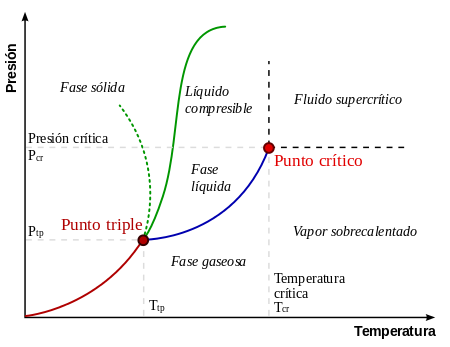
\includegraphics[width=0.55\linewidth]{ELV simple/diag_fases.png}
    \caption{Diagrama $p-T$ de una sustancia arbitraria}
    \label{fig:enter-label}
\end{figure}

En un diagrama $p-T$ la línea que separa dos fases $\alpha$ y $\beta$ se denomina curva de coexistencia. La ecuación de Clausius-Clapeyron es especialmente útil para el estudio de estas curvas, ya que relaciona la pendiente de la curva en cada punto con magnitudes que caracterizan el cambio de fase desde un punto de vista macroscópico, como la variación de entalpía o de volumen:

\begin{equation}
    \frac{dp}{dT} =\frac{\Delta h^{\alpha \to \beta}}{T\Delta v^{\alpha \to \beta}}
\end{equation}

Donde $\Delta h^{\alpha \to \beta}$ y $\Delta v^{\alpha \to \beta}$ son las variaciones de volumen molar y entalpía molar que experimenta el sistema en el cambio de fase isobárico e isotérmico de $\alpha$ a $\beta$. La curva que vamos a estudiar durante esta práctica es la de equilibrio entre la fase líquida y vapor, que tiene la característica de que $\Delta h^{\alpha \to \beta}=l^v$, como vamos a demostrar a continuación partiendo del primer principio de la termodinámica:

\begin{equation}
    \begin{gathered}
    h = u + pv \Rightarrow \dd h = \dd q - p\dd v + p\dd v + v\dd p = \dd q \\
    \Delta h^{\alpha \to \beta} = q \equiv l^v
    \end{gathered}
\end{equation}

Donde estamos trabajando siempre con magnitudes molares. Además de eso, debemos destacar que $\dd p=0$ al estar trabajando en un cambio de estado, que se dan a presión y a temperatura constante.

Para obtener una expresión útil a partir de la ecuación de Clausius-Clapeyron debemos eliminar del todo las magnitudes extensivas, más difíciles de medir. En concreto, para eliminar el volumen vamos a realizar dos aproximaciones, que el volumen del líquido es despreciable frente al del gas ($v^{vap}>>v^{liq}$) y que el gas se comporta como un gas ideal, para poder eliminar la dependencia del volumen en favor de la presión y la temperatura, magnitudes que vamos a poder medir en el laboratorio:

\begin{equation}
    \begin{gathered}
        \Delta v^{l\to v} = v^v - v^l \simeq v^v \simeq \frac{RT}{p}\\
        \frac{dp}{dT} = \frac{l^v p}{RT^2}
    \end{gathered}
\end{equation}

Donde $R$ es la constante de los gases ideales. Para obtener una expresión funcional para $p(T)$ con la que poder trabajar solo tenemos que integrar en ambas magnitudes:

\begin{equation}
    \ln p = a - \frac{l^v}{R}\frac{1}{T}
    \label{ln p}
\end{equation}

Donde $a$ es la constante de integración, que podríamos determinar con un punto de referencia $(p_0,T_0)$. Esta es una primera aproximación a la relación entre la presión y la temperatura, con la que vamos a trabajar en el laboratorio, ya que nos permite realizar una regresión lineal a una recta del tipo $\ln p = a + b/T$ para conocer el valor de $l^v$ a partir de la pendiente de la recta. Si aplicamos logaritmos a ambos lados podemos obtener una relación funcional $p(T)$:

\begin{equation}
    p(T) = e^{a-l^v/RT}
\end{equation}

No obstante, en el desarrollo matemático empleado para obtener $p(T)$ estamos aplicando una gran aproximación, que el calor de vaporización $l^v$ no depende ni de la temperatura ni de la presión, algo que en última instancia no es cierto, pero es razonable si trabajamos a temperaturas suficientemente bajas. Una mejor aproximación es considerar que los calores específicos de las fases son constantes, se puede demostrar (Adkins, 1983) que admitir esta aproximación es equivalente a considerar que el calor latente varía de forma lineal con la temperatura de la forma $l^v = l_0 + aT$. Si consideramos esta expresión podemos podemos obtener la siguiente expresión a partir de la integración de la ecuación de Clausius-Clapeyron:

\begin{equation}
    \begin{gathered}
    \ln p = \frac{a}{R} \ln T - \frac{l_0}{R}\frac{1}{T} + c \\
    p(T) = T^{a/R} e^{c-l_0/RT}
    \label{l lineal}
    \end{gathered}
\end{equation}

Donde $c$ es la constante de integración, que al igual que antes se puede calcular con un punto de referencia $(p_0,T_0)$. Pese a esto, durante la práctica vamos a considerar $l^v$ como constante por simplicidad, tomando como valor de referencia el valor tabulado a $1\;bar$ para cada substancia.

\section{Materiales y metodología}

Para el desarrollo de la práctica en el laboratorio contamos con dos cámaras de ebullición $(1,1^{\prime})$, con agua y etanol puro, donde estableceremos los respectivos equilibrios entre la fase líquida y vapor. Antes del comienzo de la práctica estas se le realizará un vacío a estas cámaras para evitar la presencia de presiones residuales que puedan afectar a los resultados, para ello se conectará una bomba de vacío en las salidas $(2,2^{\prime})$. Las cámaras de ebullición cuentan con sus respectivos sensores de presión $(3,3^{\prime})$, unidos a un manómetro digital externo $(4)$ para medir las presiones en el interior. Antes de la unión con el manómetro estos sensores deben pasar por un baño de agua fría $(6)$ para que las altas temperaturas del interior de las cámaras no produzca daños en el manómetro. Además de eso cuentan con sus respectivas sondas $(7,7^{\prime})$ conectadas unos medidores de temperatura digitales externos $(8,8^{\prime})$ para medir la temperatura en el interior. Para calentar las cámaras de ebullición contamos con dos calefactores eléctricos $(9)$ sobre los que se encuentran apoyadas las cámaras. En la siguiente figura podemos observar el montaje experimental empleado:

\begin{figure}[h!]
    \centering
    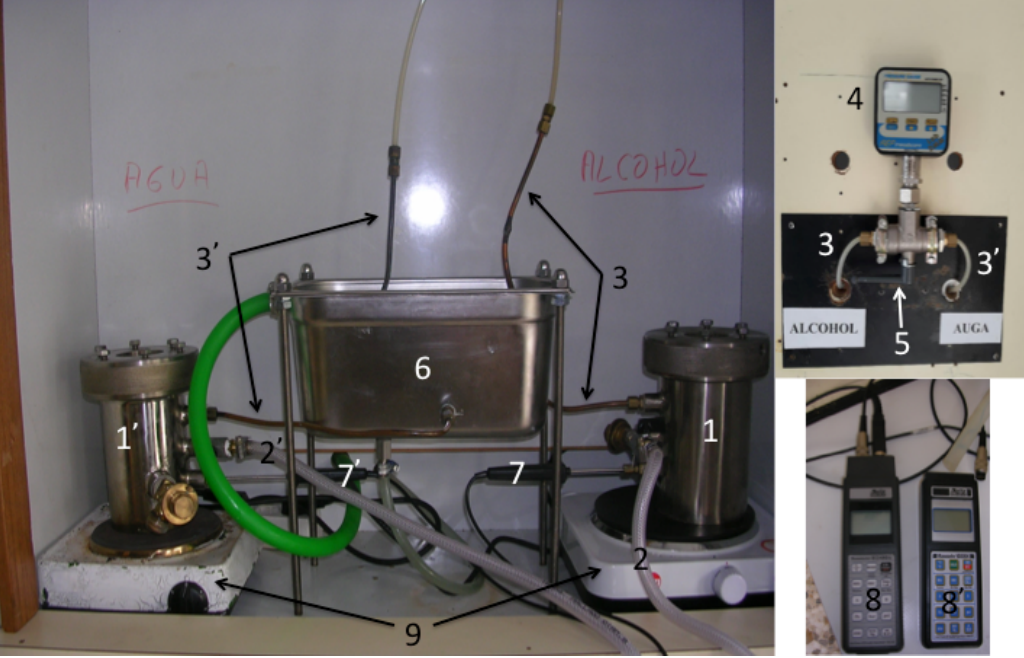
\includegraphics[width=0.65\linewidth]{ELV simple/material.png}
    \caption{Montaje experimental}
    \label{fig:enter-label}
\end{figure}

A continuación vamos a detallar el procedimiento experimental seguido en el laboratorio, que resulta ser el mismo trabajando con agua o con etanol:

\begin{enumerate}
    \item Encendemos el calentador eléctrico de la substancia con la que estemos trabajando y preparamos el manómetro para medir la presión en esa cámara, así como el medidor de temperatura.
    \item Una vez el calentador esté encendido la temperatura y la presión en el interior de la cámara comenzarán a aumentar, en ese momento comenzaremos a tomar nuestras medidas de $(p,T)$ cada vez que la temperatura aumente dos grados. Cuando la presión alcance los 5 bares desconectaremos el calefactor y finalizaremos la toma de medidas del calentamiento.
    \item Tras un cierto tiempo la temperatura y la presión comenzarán a bajar. En este momento comenzaremos la segunda toma de medidas de $(p,T)$, que constituirán una muestra independiente a la primera. Cuando la temperatura alcance los $80 \;^{\circ}C$ daremos por finalizada la toma de datos.
    \item Repetimos la experiencia con la otra substancia
\end{enumerate}

\newpage

Los datos medidos son de presión y temperatura, medidos ambos con medidores digitales de forma directa, por lo que su incertidumbre vendrá dada por la precisión experimental del aparato. En el caso de la presión decidimos dotarle algo más de incertidumbre por las fluctuaciones observadas durante la toma de medidas.

\begin{equation}
    s(T) = 0,1 \; ^{\circ}C \quad s(p) = 0,005 \;bar
\end{equation}

\section{Resultados experimentales y tratamiento de datos}

Para el tratamiento de datos trabajaremos inicialmente con la ecuación \ref{ln p}, que nos permitirá ajustar los datos a una recta de regresión del tipo $\ln p = a + b/T$, como ya hemos mencionado antes. La pendiente de la recta de regresión será la que nos proporcione el valor de $l^v$ de forma trivial. No obstante, antes de hacer la regresión tenemos que expresar nuestras medidas de la forma en que las vamos a emplear con sus respectivas incertidumbres. Los valores de $\ln p$ y $1/T$ empleados figurarán en la tabla de datos en el anexo. Sus incertidumbres se pueden obtener por propagación a partir de las siguientes expresiones:

\begin{equation}
    s(\ln p) = \frac{s(p)}{p} \quad s(1/T) = \frac{s(T)}{T^2}
\end{equation}

Una vez tengamos nuestras magnitudes expresadas correctamente podemos proceder a realizar las diferentes regresiones para cada una de las substancias:

\subsection{Etanol}

Los resultados de los ajustes de $\ln p = a + b/T$ son los siguientes:

\begin{figure}[h!]
    \centering
    \begin{subfigure}{0.49\textwidth}
        \centering
        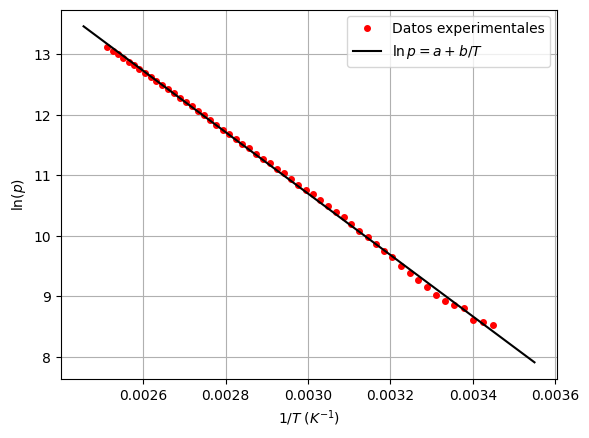
\includegraphics[width=1.05\linewidth]{ELV simple/cal_oh.png}
        \subcaption{Calentamiento}
    \end{subfigure}
    \begin{subfigure}{0.49\textwidth}
        \centering
        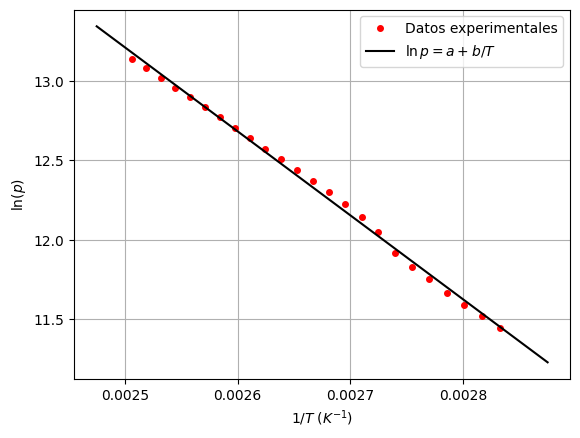
\includegraphics[width=1.05\linewidth]{ELV simple/enf_oh.png}
        \subcaption{Enfriamiento}
    \end{subfigure}
    \caption{Datos experimentales y ajuste $\ln p = a + b/T$}
    \label{fig:enter-label}
\end{figure}

\begin{table}[h!]
\centering
\begin{tabular}{c|c|c|}
\cline{2-3}
                                  & Calentamiento & Enfriamiento \\ \hline
\multicolumn{1}{|c|}{$a$}         & $25,898$ & $26,40$ \\ \hline
\multicolumn{1}{|c|}{$b\;(K)$}    & $-5067$ & $-5276$ \\ \hline
\multicolumn{1}{|c|}{$s(a)$}      & $0,056$ & $0,17$ \\ \hline
\multicolumn{1}{|c|}{$s(b)\;(K)$} & $19$ & $22$ \\ \hline
\multicolumn{1}{|c|}{$r$}         & $-0,9996$ & $-0,998$ \\ \hline
\end{tabular}
\caption{Datos de las regresiones de $\ln p$ frente a $1/T$ para el etanol}
\label{tab:my-table}
\end{table}

A partir de los datos de las regresiones podemos calcular $l^v$ de forma muy sencilla comparando la ecuación de la recta de regresión con la expresión obtenida a partir de la integración de la ecuación de Clausius-Clapeyron (\ref{ln p}):

\begin{equation}
    b = -\frac{l^v}{R} \Rightarrow l^v = -b\cdot R \quad s(l^v) = R\cdot s(b)
    \label{s_l^v}
\end{equation}

El resultado de $l^v$ obtenido va a depender de las unidades empleadas en la constante de los gases ideales, $R$. En nuestro cálculo vamos a considerar $R=8,314 \;J/mol\cdot K$, en unidades del sistema internacional. Por tanto, el valor obtenido para $l^v$ va a tener unidades de $J/mol$, para expresarlo en función de la masa y no de los moles solo tenemos que dividir el resultado entre la masa molar de la substancia. En la siguiente tabla podemos ver los valores de $l^v$ obtenidos:

\begin{table}[h!]
\centering
\begin{tabular}{c|c|c|}
\cline{2-3}
    & Calentamiento & Enfriamiento \\ \hline
\multicolumn{1}{|c|}{$l^v\;(kJ/kg)$}    & $914,5$ & $952$ \\ \hline
\multicolumn{1}{|c|}{$s(l^v)\;(kJ/kg)$} & $3,4$ & $11$ \\ \hline
\end{tabular}
\caption{Calores de vaporización obtenidos con el etanol}
\label{tab:my-table}
\end{table}

Para comprobar la validez de los resultados vamos a considerar como valor de referencia el valor de $l^v$ tabulado a una presión de $1\; bar$, ara el etanol $l^v$ a $1\;bar$ tiene un valor de $841\; kJ/kg$. Comparando con este valor, podemos ver que los resultados obtenidos se encuentran ambos un poco por encima de lo esperado, sobre todo el de la serie de medidas de enfriamiento. Teniendo en cuenta estos resultados podemos pensar en dos posibles problemáticas que afectaron a nuestros resultados, que la presión medida es menor que la esperada o que la temperatura medida es mayor que la esperada. No obstante, esperaremos a las conclusiones para considerar todos los valores obtenidos de $l^v$ y veremos si este error es sistemático o afecta solo a las medidas del etanol.

\subsection{Agua}

Los resultados de los ajustes de $\ln p = a + b/T$ son los siguientes:

\begin{figure}[h!]
    \centering
    \begin{subfigure}{0.49\textwidth}
        \centering
        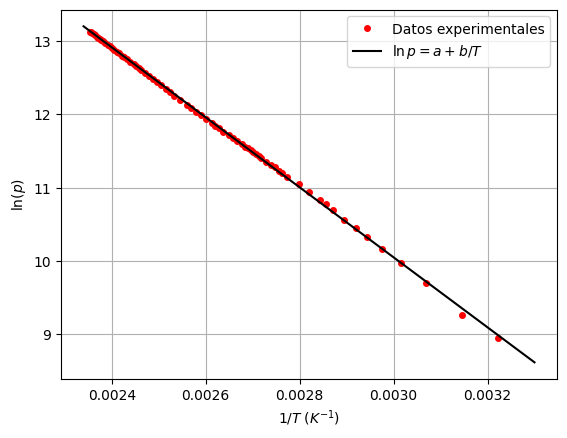
\includegraphics[width=1\linewidth]{ELV simple/cal_agua.png}
        \subcaption{Calentamiento}
    \end{subfigure}
    \begin{subfigure}{0.49\textwidth}
        \centering
        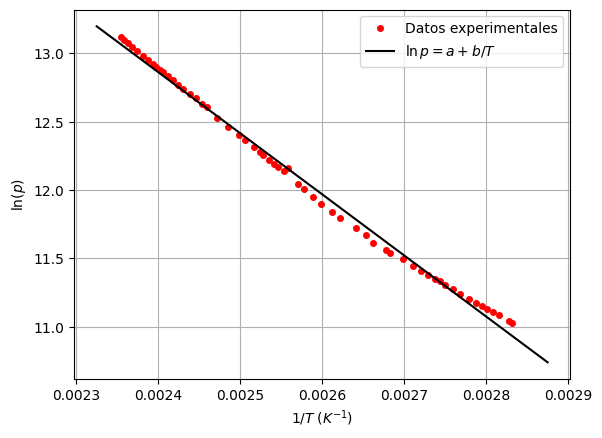
\includegraphics[width=1.05\linewidth]{ELV simple/enf_agua.png}
        \subcaption{Enfriamiento}
    \end{subfigure}
    \caption{Datos experimentales y ajuste $\ln p = a + b/T$}
    \label{fig:enter-label}
\end{figure}

\begin{table}[h!]
\centering
\begin{tabular}{c|c|c|}
\cline{2-3}
    & Calentamiento & Enfriamiento \\ \hline
\multicolumn{1}{|c|}{$a$}         & $24,352$ & $23,58$ \\ \hline
\multicolumn{1}{|c|}{$b\;(K)$}    & $-4767$ & $-4465$ \\ \hline
\multicolumn{1}{|c|}{$s(a)$}      & $0,057$ & $0,10$ \\ \hline
\multicolumn{1}{|c|}{$s(b)\;(K)$} & $22$ & $40$ \\ \hline
\multicolumn{1}{|c|}{$r$}         & $-0,9992$ & $-0,997$ \\ \hline
\end{tabular}
\caption{Datos de las regresiones de $\ln p$ frente a $1/T$ para el agua}
\label{tab:my-table}
\end{table}

Una vez tenemos los parámetros de las regresiones lineales el procedimiento para obtener $l^v$ es idéntico al que seguimos con el etanol, empleando las ecuaciones (\ref{ln p}) y (\ref{s_l^v}). En la siguiente tabla podemos ver los resultados obtenidos:

\begin{table}[h!]
\centering
\begin{tabular}{c|c|c|}
\cline{2-3}
                                       & Calentamiento & Enfriamiento \\ \hline
\multicolumn{1}{|c|}{$l^v\;(kJ/kg)$}    & $2196,5$ & $2062$ \\ \hline
\multicolumn{1}{|c|}{$s(l^v)\;(kJ/kg)$} & $4,9$ & $18$ \\ \hline
\end{tabular}
\caption{Calores de vaporización obtenidos con el agua}
\label{tab:my-table}
\end{table}

Al igual que con el etanol, para comprobar la validez de los resultados vamos a considerar como valor de referencia el calor de vaporización del agua a una presión de $1\;bar$, que resulta ser de $2257\;kJ/kg$. En este caso los valores obtenidos a partir de las regresiones son inferiores a lo esperado, por lo que no podemos afirmar que exista un error sistemático en el experimento. En este caso, al ser el resultado inferior al esperado podemos pensar que el vacío de las cámaras de ebullición no fue perfecto y que existían ciertas presiones residuales que provocaban que la presión medida fuera menor de lo esperado.

\subsection{Curvas de coexistencia}

Como ya hemos detallado durante la introducción teórica, si aplicamos exponenciales a la ecuación \ref{ln p}, obtenida a partir de integrar la ecuación de Clausius-Clapeyron, podemos obtener una expresión analítica de $p(T)$. Esta expresión se corresponde con la ecuación de la curva de coexistencia de las fases líquida y vapor y a partir de ella podemos obtener el calor de vaporización con un ajuste exponencial como el siguiente:

\begin{equation}
    p(T) = e^{a-l^v/RT} = e^{a}e^{-l^v/RT} \sim ce^{b/T}
    \label{p(T)}
\end{equation}

Donde $c$ y $b$ son los parámetros a ajustar. A continuación vamos a exponer brevemente los resultados de este ajuste exponencial para ambas substancias.

\subsubsection{Etanol}

En la siguiente figura podemos ver las curvas de coexistencia obtenidas a partir del ajuste exponencial para el etanol:

\begin{figure}[h!]
    \centering
    \begin{subfigure}{0.49\textwidth}
        \centering
        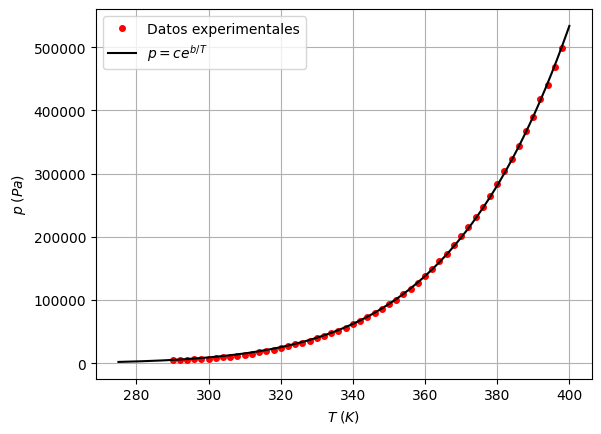
\includegraphics[width=1.02\linewidth]{ELV simple/curva_c_oh.png}
        \subcaption{Calentamiento}
    \end{subfigure}
    \begin{subfigure}{0.49\textwidth}
        \centering
        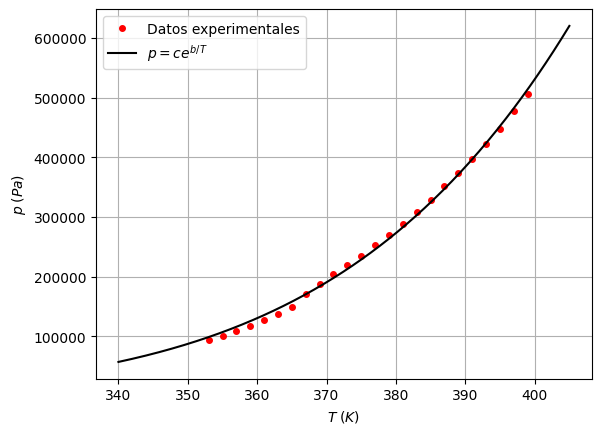
\includegraphics[width=1.02\linewidth]{ELV simple/curva_e_oh.png}
        \subcaption{Enfriamiento}
    \end{subfigure}
    \caption{Datos experimentales y ajuste $p=ce^{b/T}$}
    \label{fig:enter-label}
\end{figure}

El valor de $l^v$ se puede obtener de forma sencilla a partir de los parámetros de la regresión:

\begin{equation}
    b = -\frac{l^v}{R} \Rightarrow l^v = -b\cdot R \quad s(l^v) = R \cdot s(b)
    \label{inc_l^v_2}
\end{equation}

En la siguiente tabla expondremos los resultados de las regresiones, así como el valor de $l^v$ obtenido a partir de ellas con su incertidumbre:

\begin{table}[h!]
\centering
\begin{tabular}{c|c|c|}
\cline{2-3}
    & Calentamiento       & Enfriamiento                    \\ \hline
\multicolumn{1}{|c|}{$c \pm s(c) \;(Pa)$} & $(1,030 \pm 0,031) \cdot 10^{11}$ & $(1,61\pm 0,25) \cdot 10^{11}$  \\ \hline
\multicolumn{1}{|c|}{$b \pm s(b) \; (K)$} & $-4868 \pm 15$   & $5049 \pm 61 $ \\ \hline
\multicolumn{1}{|c|}{$l^v\;(kJ/kg)$}       & 878,6                             & 911                             \\ \hline
\multicolumn{1}{|c|}{$s(l^v)\;(kJ/kg)$}    & 2,1                               & 11                              \\ \hline
\end{tabular}
\caption{Calores de vaporización obtenidos con el ajuste exponencial para el etanol}
\label{tab:my-table}
\end{table}

Es interesante observar que los resultados obtenidos con el ajuste exponencial son mucho mejores que con el lineal, los valores de $l^v$ están mucho más cerca del valor que tomamos como referencia, de $841 \;KJ/kg$.

\newpage

\subsubsection{Agua}

En la siguiente figura podemos ver las curvas de coexistencia obtenidas con los ajustes exponenciales de los datos del agua:

\begin{figure}[h!]
    \centering
    \begin{subfigure}{0.49\textwidth}
        \centering
        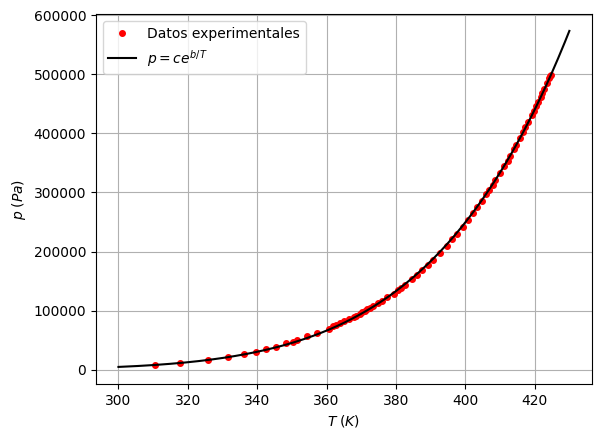
\includegraphics[width=1.02\linewidth]{ELV simple/curva_c_agua.png}
        \subcaption{Calentamiento}
    \end{subfigure}
    \begin{subfigure}{0.49\textwidth}
        \centering
        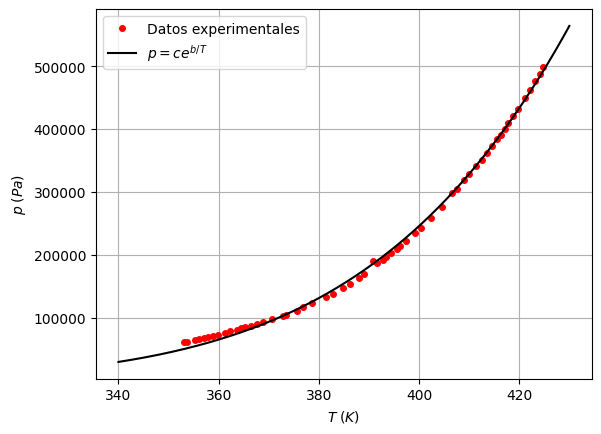
\includegraphics[width=1.02\linewidth]{ELV simple/curva_e_agua.png}
        \subcaption{Enfriamiento}
    \end{subfigure}
    \caption{Datos experimentales y ajuste $p=ce^{b/T}$}
    \label{fig:enter-label}
\end{figure}

El procedimiento para obtener $l^v$ a partir de los datos de los ajuste es análogo al del etanol, empleando la Ec.\ref{inc_l^v_2}. En la siguiente tabla podemos ver los valores de los parámetros del ajuste y del calor de vaporización del agua:

\begin{table}[h!]
\centering
\begin{tabular}{c|c|c|}
\cline{2-3}
    & Calentamiento   & Enfriamiento                    \\ \hline
\multicolumn{1}{|c|}{$c \pm s(c) \;(Pa)$} & $(3,825 \pm 0,077) \cdot 10^{10}$ & $(3,58 \pm 0,28) \cdot 10^{10}$ \\ \hline
\multicolumn{1}{|c|}{$b \pm s(b) \; (K)$} & $-4776,5 \pm 8,3$                 & $-4756 \pm 32$                  \\ \hline
\multicolumn{1}{|c|}{$l^v\;(kJ/kg)$}       & 2206,2                            & 2197                            \\ \hline
\multicolumn{1}{|c|}{$s(l^v)\;(kJ/kg)$}    & 3,8                               & 15                              \\ \hline
\end{tabular}
\caption{Calores de vaporización obtenidos con el ajuste exponencial para el agua}
\label{tab:my-table}
\end{table}

Al igual que con el etanol, los resultados para $l^v$ son más adecuados al valor de referencia, de $2257 \; kJ/kg$ para el agua, con el ajuste exponencial que con el ajuste lineal.


\subsection{Análisis estadístico}

Como ya hemos mencionado anteriormente, tenemos dos muestras estadísticamente independiente para cada substancia, las medidas tomadas durante la subida y la bajada de las temperaturas. Esto nos permitirá realizar un pequeño tratamiento estadístico de los datos, para obtener un valor de $l^v$ de cada substancia que comparar con el teórico. Para ello el procedimiento llevado a cabo fue calcular la media ponderada entre el resultado del calentamiento y del enfriamiento para las dos regresiones, lineal y exponencial. Para ello empleamos las siguientes fórmulas. Como incertidumbre del resultado tomaremos la desviación típica, resultados que vendrán dados por las siguientes fórmulas:

\begin{equation}
    \begin{gathered}
        \bar{l^v} = \frac{l^v_c w_c + l^v_e w_e}{w_c+w_e} \\
        s(\bar{l^v}) = \frac{1}{\sqrt{w_c + w_e}} \\
        w_c = \frac{1}{s(l^v_c)^2} \quad w_e = \frac{1}{s(l^v_e)^2}
    \end{gathered}
\end{equation}

En la siguiente tabla podemos ver los resultados finales de los calores de vaporización para los dos ajustes:

\begin{table}[h!]
\centering
\begin{tabular}{|c|c|c|}
\hline
$l^v \pm s(l^v)\; (kJ/kg)$ & Etanol & Agua \\ \hline
Referencia       & 841 & 2257 \\ \hline
Lineal           & $917,6 \pm 3,3$ & $2187,6 \pm 4,7$ \\ \hline
Exponencial      & $879,7 \pm 2,0$ & $2205,6 \pm 3,7$ \\ \hline
\end{tabular}
\caption{Resultados del análisis estadístico}
\label{tab:my-table}
\end{table}

A la vista de los resultados podemos ver que la media ponderada representa un buen estimador del valor real, pues le da mucha más importancia a los datos del calentamiento, que tienen una incertidumbre mucho menor y se corresponden más con la realidad. Por otro lado, podemos ver otra vez que los resultados de las regresiones exponenciales se corresponden mucho más con los valores de referencia, algo que ya habíamos observado antes.


\section{Conclusiones}

Tras realizar el análisis estadístico de los resultados podemos realizar unas conclusiones con más rigurosidad. Los resultados son bastante consistentes para ambas substancias, queda reflejado que el análisis exponencial proporciona resultados mucho más acertados y próximos al valor de referencia. Además de eso pudimos ver que los datos de las series en las que bajaba la temperatura presentan una incertidumbre mayor y resultados más alejados de lo esperado.

Estas desviaciones de los valores tabulados de los calores de vaporización pueden deberse a muchos factores, desde un mal funcionamiento de los aparatos de medida a un cierto error generado por las aproximaciones realizadas. Considerar la fase vapor como un gas ideal puede llevar a cierto error, especialmente a temperaturas elevadas, para minimizarlo y obtener mejores resultados podemos pensar en emplear modelos como el de Van der Waals para los gases reales, pero que podría complicar la integración de la ecuación de Clausius-Clapeyron.

\section{Bibliografía}

\begin{itemize}
    \item \textit{Diagrama de fase}. https://es.wikipedia.org/wiki/Diagrama\_de\_fase
    \item Adkins, C. J. (1983). \textit{Equilibrium Thermodynamics}. Cambridge University Press.
    \item Carlos Rey Losada, \textit{Apuntes de la asignatura Fundamentos de la termodinámica}
\end{itemize}

\newpage

\section{Anexo: Tablas de datos}

Las incertidumbres de las magnitudes de las magnitudes medidas en el laboratorio son:

\begin{equation}
    s(p) = 0,005 \; Bar \quad s(T) = 0,1 \; (^{\circ}C) 
\end{equation}

\begin{table}[h!]
\centering
\begin{tabular}{|cccccc}
\hline
\multicolumn{4}{|c|}{Calentamiento}                                                                                                                      & \multicolumn{2}{c|}{Enfriamiento}                                          \\ \hline
\multicolumn{1}{|c|}{$p \;(Bar)$} & \multicolumn{1}{c|}{$T \; (^{\circ}C)$} & \multicolumn{1}{c|}{$p \;(Bar)$} & \multicolumn{1}{c|}{$T \; (^{\circ}C)$} & \multicolumn{1}{c|}{$p \;(Bar)$} & \multicolumn{1}{c|}{$T \; (^{\circ}C)$} \\ \hline
\multicolumn{1}{|c|}{0.050}        & \multicolumn{1}{c|}{17.0}               & \multicolumn{1}{c|}{0.788}       & \multicolumn{1}{c|}{73.0}               & \multicolumn{1}{c|}{5.060}        & \multicolumn{1}{c|}{126.0}              \\ \hline
\multicolumn{1}{|c|}{0.053}       & \multicolumn{1}{c|}{19.0}               & \multicolumn{1}{c|}{0.853}       & \multicolumn{1}{c|}{75.0}               & \multicolumn{1}{c|}{4.778}       & \multicolumn{1}{c|}{124.0}              \\ \hline
\multicolumn{1}{|c|}{0.055}       & \multicolumn{1}{c|}{21.0}               & \multicolumn{1}{c|}{0.930}        & \multicolumn{1}{c|}{77.0}               & \multicolumn{1}{c|}{4.481}       & \multicolumn{1}{c|}{122.0}              \\ \hline
\multicolumn{1}{|c|}{0.067}       & \multicolumn{1}{c|}{23.0}               & \multicolumn{1}{c|}{1.007}       & \multicolumn{1}{c|}{79.0}               & \multicolumn{1}{c|}{4.232}       & \multicolumn{1}{c|}{120.0}              \\ \hline
\multicolumn{1}{|c|}{0.070}        & \multicolumn{1}{c|}{25.0}               & \multicolumn{1}{c|}{1.092}       & \multicolumn{1}{c|}{81.0}               & \multicolumn{1}{c|}{3.979}       & \multicolumn{1}{c|}{118.0}              \\ \hline
\multicolumn{1}{|c|}{0.075}       & \multicolumn{1}{c|}{27.0}               & \multicolumn{1}{c|}{1.178}       & \multicolumn{1}{c|}{83.0}               & \multicolumn{1}{c|}{3.744}       & \multicolumn{1}{c|}{116.0}              \\ \hline
\multicolumn{1}{|c|}{0.083}       & \multicolumn{1}{c|}{29.0}               & \multicolumn{1}{c|}{1.270}        & \multicolumn{1}{c|}{85.0}               & \multicolumn{1}{c|}{3.513}       & \multicolumn{1}{c|}{114.0}              \\ \hline
\multicolumn{1}{|c|}{0.094}       & \multicolumn{1}{c|}{31.0}               & \multicolumn{1}{c|}{1.380}        & \multicolumn{1}{c|}{87.0}               & \multicolumn{1}{c|}{3.293}       & \multicolumn{1}{c|}{112.0}              \\ \hline
\multicolumn{1}{|c|}{0.106}       & \multicolumn{1}{c|}{33.0}               & \multicolumn{1}{c|}{1.494}       & \multicolumn{1}{c|}{89.0}               & \multicolumn{1}{c|}{3.082}       & \multicolumn{1}{c|}{110.0}              \\ \hline
\multicolumn{1}{|c|}{0.119}       & \multicolumn{1}{c|}{35.0}               & \multicolumn{1}{c|}{1.615}       & \multicolumn{1}{c|}{91.0}               & \multicolumn{1}{c|}{2.886}       & \multicolumn{1}{c|}{108.0}              \\ \hline
\multicolumn{1}{|c|}{0.134}       & \multicolumn{1}{c|}{37.0}               & \multicolumn{1}{c|}{1.732}       & \multicolumn{1}{c|}{93.0}               & \multicolumn{1}{c|}{2.700}         & \multicolumn{1}{c|}{106.0}              \\ \hline
\multicolumn{1}{|c|}{0.154}       & \multicolumn{1}{c|}{39.0}               & \multicolumn{1}{c|}{1.865}       & \multicolumn{1}{c|}{95.0}               & \multicolumn{1}{c|}{2.524}       & \multicolumn{1}{c|}{104.0}              \\ \hline
\multicolumn{1}{|c|}{0.172}       & \multicolumn{1}{c|}{41.0}               & \multicolumn{1}{c|}{2.010}        & \multicolumn{1}{c|}{97.0}               & \multicolumn{1}{c|}{2.355}       & \multicolumn{1}{c|}{102.0}              \\ \hline
\multicolumn{1}{|c|}{0.191}       & \multicolumn{1}{c|}{43.0}               & \multicolumn{1}{c|}{2.154}       & \multicolumn{1}{c|}{99.0}               & \multicolumn{1}{c|}{2.196}       & \multicolumn{1}{c|}{100.0}              \\ \hline
\multicolumn{1}{|c|}{0.217}       & \multicolumn{1}{c|}{45.0}               & \multicolumn{1}{c|}{2.308}       & \multicolumn{1}{c|}{101.0}              & \multicolumn{1}{c|}{2.043}       & \multicolumn{1}{c|}{98.0}               \\ \hline
\multicolumn{1}{|c|}{0.238}       & \multicolumn{1}{c|}{47.0}               & \multicolumn{1}{c|}{2.468}       & \multicolumn{1}{c|}{103.0}              & \multicolumn{1}{c|}{1.872}       & \multicolumn{1}{c|}{96.0}               \\ \hline
\multicolumn{1}{|c|}{0.269}       & \multicolumn{1}{c|}{49.0}               & \multicolumn{1}{c|}{2.643}       & \multicolumn{1}{c|}{105.0}              & \multicolumn{1}{c|}{1.704}       & \multicolumn{1}{c|}{94.0}               \\ \hline
\multicolumn{1}{|c|}{0.298}       & \multicolumn{1}{c|}{51.0}               & \multicolumn{1}{c|}{2.838}       & \multicolumn{1}{c|}{107.0}              & \multicolumn{1}{c|}{1.498}       & \multicolumn{1}{c|}{92.0}               \\ \hline
\multicolumn{1}{|c|}{0.328}       & \multicolumn{1}{c|}{53.0}               & \multicolumn{1}{c|}{3.039}       & \multicolumn{1}{c|}{109.0}              & \multicolumn{1}{c|}{1.375}       & \multicolumn{1}{c|}{90.0}               \\ \hline
\multicolumn{1}{|c|}{0.360}        & \multicolumn{1}{c|}{55.0}               & \multicolumn{1}{c|}{3.238}       & \multicolumn{1}{c|}{111.0}              & \multicolumn{1}{c|}{1.268}       & \multicolumn{1}{c|}{88.0}               \\ \hline
\multicolumn{1}{|c|}{0.397}       & \multicolumn{1}{c|}{57.0}               & \multicolumn{1}{c|}{3.432}       & \multicolumn{1}{c|}{113.0}              & \multicolumn{1}{c|}{1.166}       & \multicolumn{1}{c|}{86.0}               \\ \hline
\multicolumn{1}{|c|}{0.435}       & \multicolumn{1}{c|}{59.0}               & \multicolumn{1}{c|}{3.671}       & \multicolumn{1}{c|}{115.0}              & \multicolumn{1}{c|}{1.082}       & \multicolumn{1}{c|}{84.0}               \\ \hline
\multicolumn{1}{|c|}{0.472}       & \multicolumn{1}{c|}{61.0}               & \multicolumn{1}{c|}{3.901}       & \multicolumn{1}{c|}{117.0}              & \multicolumn{1}{c|}{1.007}       & \multicolumn{1}{c|}{82.0}               \\ \hline
\multicolumn{1}{|c|}{0.513}       & \multicolumn{1}{c|}{63.0}               & \multicolumn{1}{c|}{4.175}       & \multicolumn{1}{c|}{119.0}              & \multicolumn{1}{c|}{0.935}       & \multicolumn{1}{c|}{80.0}               \\ \hline
\multicolumn{1}{|c|}{0.564}       & \multicolumn{1}{c|}{65.0}               & \multicolumn{1}{c|}{4.408}       & \multicolumn{1}{c|}{121.0}              &                                  &                                         \\ \cline{1-4}
\multicolumn{1}{|c|}{0.616}       & \multicolumn{1}{c|}{67.0}               & \multicolumn{1}{c|}{4.689}       & \multicolumn{1}{c|}{123.0}              &                                  &                                         \\ \cline{1-4}
\multicolumn{1}{|c|}{0.668}       & \multicolumn{1}{c|}{69.0}               & \multicolumn{1}{c|}{4.989}       & \multicolumn{1}{c|}{125.0}              &                                  &                                         \\ \cline{1-4}
\multicolumn{1}{|c|}{0.727}       & \multicolumn{1}{c|}{71.0}               &                                  &                                         &                                  &                                         \\ \cline{1-2}
\end{tabular}
\caption{Datos experimentales tomados en el laboratorio para el etanol}
\label{tab:my-table}
\end{table}

\newpage

\begin{table}[]
\centering
\begin{tabular}{|cccccccc}
\hline
\multicolumn{4}{|c|}{Calentamiento}                                                                                                                      & \multicolumn{4}{c|}{Enfriamiento}                                                                                                                       \\ \hline
\multicolumn{1}{|c|}{$p \;(Bar)$} & \multicolumn{1}{c|}{$T \; (^{\circ}C)$} & \multicolumn{1}{c|}{$p \;(Bar)$} & \multicolumn{1}{c|}{$T \; (^{\circ}C)$} & \multicolumn{1}{c|}{$p \;(Bar)$} & \multicolumn{1}{c|}{$T \; (^{\circ}C)$} & \multicolumn{1}{c|}{$p \;(Bar)$} & \multicolumn{1}{c|}{$T \; (^{\circ}C)$} \\ \hline
\multicolumn{1}{|c|}{0.077}       & \multicolumn{1}{c|}{37.4}               & \multicolumn{1}{c|}{1.772}       & \multicolumn{1}{c|}{116.2}              & \multicolumn{1}{c|}{4.986}       & \multicolumn{1}{c|}{151.8}              & \multicolumn{1}{c|}{1.907}       & \multicolumn{1}{c|}{117.8}              \\ \hline
\multicolumn{1}{|c|}{0.106}       & \multicolumn{1}{c|}{44.8}               & \multicolumn{1}{c|}{1.853}       & \multicolumn{1}{c|}{117.7}              & \multicolumn{1}{c|}{4.881}       & \multicolumn{1}{c|}{151.1}              & \multicolumn{1}{c|}{1.705}       & \multicolumn{1}{c|}{116.1}              \\ \hline
\multicolumn{1}{|c|}{0.163}       & \multicolumn{1}{c|}{52.8}               & \multicolumn{1}{c|}{1.980}       & \multicolumn{1}{c|}{119.8}              & \multicolumn{1}{c|}{4.765}       & \multicolumn{1}{c|}{150.2}              & \multicolumn{1}{c|}{1.638}       & \multicolumn{1}{c|}{115.0}              \\ \hline
\multicolumn{1}{|c|}{0.214}       & \multicolumn{1}{c|}{58.7}               & \multicolumn{1}{c|}{2.098}       & \multicolumn{1}{c|}{121.7}              & \multicolumn{1}{c|}{4.626}       & \multicolumn{1}{c|}{149.2}              & \multicolumn{1}{c|}{1.543}       & \multicolumn{1}{c|}{113.2}              \\ \hline
\multicolumn{1}{|c|}{0.26}        & \multicolumn{1}{c|}{63.1}               & \multicolumn{1}{c|}{2.210}       & \multicolumn{1}{c|}{123.3}              & \multicolumn{1}{c|}{4.487}       & \multicolumn{1}{c|}{148.1}              & \multicolumn{1}{c|}{1.473}       & \multicolumn{1}{c|}{111.8}              \\ \hline
\multicolumn{1}{|c|}{0.305}       & \multicolumn{1}{c|}{66.7}               & \multicolumn{1}{c|}{2.300}       & \multicolumn{1}{c|}{124.7}              & \multicolumn{1}{c|}{4.326}       & \multicolumn{1}{c|}{146.8}              & \multicolumn{1}{c|}{1.388}       & \multicolumn{1}{c|}{109.9}              \\ \hline
\multicolumn{1}{|c|}{0.346}       & \multicolumn{1}{c|}{69.4}               & \multicolumn{1}{c|}{2.422}       & \multicolumn{1}{c|}{126.3}              & \multicolumn{1}{c|}{4.206}       & \multicolumn{1}{c|}{145.8}              & \multicolumn{1}{c|}{1.327}       & \multicolumn{1}{c|}{108.4}              \\ \hline
\multicolumn{1}{|c|}{0.387}       & \multicolumn{1}{c|}{72.4}               & \multicolumn{1}{c|}{2.525}       & \multicolumn{1}{c|}{127.7}              & \multicolumn{1}{c|}{4.090}       & \multicolumn{1}{c|}{144.8}              & \multicolumn{1}{c|}{1.232}       & \multicolumn{1}{c|}{105.6}              \\ \hline
\multicolumn{1}{|c|}{0.443}       & \multicolumn{1}{c|}{75.3}               & \multicolumn{1}{c|}{2.646}       & \multicolumn{1}{c|}{129.1}              & \multicolumn{1}{c|}{4.009}       & \multicolumn{1}{c|}{144.1}              & \multicolumn{1}{c|}{1.169}       & \multicolumn{1}{c|}{103.9}              \\ \hline
\multicolumn{1}{|c|}{0.476}       & \multicolumn{1}{c|}{77.2}               & \multicolumn{1}{c|}{2.745}       & \multicolumn{1}{c|}{130.5}              & \multicolumn{1}{c|}{3.913}       & \multicolumn{1}{c|}{143.3}              & \multicolumn{1}{c|}{1.105}       & \multicolumn{1}{c|}{102.7}              \\ \hline
\multicolumn{1}{|c|}{0.509}       & \multicolumn{1}{c|}{78.6}               & \multicolumn{1}{c|}{2.858}       & \multicolumn{1}{c|}{131.7}              & \multicolumn{1}{c|}{3.843}       & \multicolumn{1}{c|}{142.6}              & \multicolumn{1}{c|}{1.053}       & \multicolumn{1}{c|}{100.4}              \\ \hline
\multicolumn{1}{|c|}{0.567}       & \multicolumn{1}{c|}{81.5}               & \multicolumn{1}{c|}{2.970}       & \multicolumn{1}{c|}{133.0}              & \multicolumn{1}{c|}{3.735}       & \multicolumn{1}{c|}{141.6}              & \multicolumn{1}{c|}{1.029}       & \multicolumn{1}{c|}{99.8}               \\ \hline
\multicolumn{1}{|c|}{0.627}       & \multicolumn{1}{c|}{84.2}               & \multicolumn{1}{c|}{3.047}       & \multicolumn{1}{c|}{133.9}              & \multicolumn{1}{c|}{3.626}       & \multicolumn{1}{c|}{140.6}              & \multicolumn{1}{c|}{0.979}       & \multicolumn{1}{c|}{97.6}               \\ \hline
\multicolumn{1}{|c|}{0.692}       & \multicolumn{1}{c|}{87.6}               & \multicolumn{1}{c|}{3.127}       & \multicolumn{1}{c|}{134.9}              & \multicolumn{1}{c|}{3.514}       & \multicolumn{1}{c|}{139.5}              & \multicolumn{1}{c|}{0.935}       & \multicolumn{1}{c|}{95.9}               \\ \hline
\multicolumn{1}{|c|}{0.735}       & \multicolumn{1}{c|}{89.0}               & \multicolumn{1}{c|}{3.204}       & \multicolumn{1}{c|}{135.7}              & \multicolumn{1}{c|}{3.415}       & \multicolumn{1}{c|}{138.4}              & \multicolumn{1}{c|}{0.900}       & \multicolumn{1}{c|}{94.6}               \\ \hline
\multicolumn{1}{|c|}{0.755}       & \multicolumn{1}{c|}{89.8}               & \multicolumn{1}{c|}{3.330}       & \multicolumn{1}{c|}{137.0}              & \multicolumn{1}{c|}{3.293}       & \multicolumn{1}{c|}{137.0}              & \multicolumn{1}{c|}{0.877}       & \multicolumn{1}{c|}{93.5}               \\ \hline
\multicolumn{1}{|c|}{0.788}       & \multicolumn{1}{c|}{91.0}               & \multicolumn{1}{c|}{3.440}       & \multicolumn{1}{c|}{138.1}              & \multicolumn{1}{c|}{3.188}       & \multicolumn{1}{c|}{135.9}              & \multicolumn{1}{c|}{0.852}       & \multicolumn{1}{c|}{92.3}               \\ \hline
\multicolumn{1}{|c|}{0.816}       & \multicolumn{1}{c|}{92.1}               & \multicolumn{1}{c|}{3.540}       & \multicolumn{1}{c|}{139.2}              & \multicolumn{1}{c|}{3.053}       & \multicolumn{1}{c|}{134.5}              & \multicolumn{1}{c|}{0.835}       & \multicolumn{1}{c|}{91.5}               \\ \hline
\multicolumn{1}{|c|}{0.853}       & \multicolumn{1}{c|}{93.4}               & \multicolumn{1}{c|}{3.620}       & \multicolumn{1}{c|}{129.9}              & \multicolumn{1}{c|}{2.978}       & \multicolumn{1}{c|}{133.5}              & \multicolumn{1}{c|}{0.815}       & \multicolumn{1}{c|}{90.6}               \\ \hline
\multicolumn{1}{|c|}{0.894}       & \multicolumn{1}{c|}{94.9}               & \multicolumn{1}{c|}{3.742}       & \multicolumn{1}{c|}{141.1}              & \multicolumn{1}{c|}{2.761}       & \multicolumn{1}{c|}{131.5}              & \multicolumn{1}{c|}{0.790}       & \multicolumn{1}{c|}{89.3}               \\ \hline
\multicolumn{1}{|c|}{0.915}       & \multicolumn{1}{c|}{95.5}               & \multicolumn{1}{c|}{3.809}       & \multicolumn{1}{c|}{141.7}              & \multicolumn{1}{c|}{2.584}       & \multicolumn{1}{c|}{129.4}              & \multicolumn{1}{c|}{0.760}       & \multicolumn{1}{c|}{88.2}               \\ \hline
\multicolumn{1}{|c|}{0.947}       & \multicolumn{1}{c|}{96.5}               & \multicolumn{1}{c|}{3.919}       & \multicolumn{1}{c|}{142.8}              & \multicolumn{1}{c|}{2.434}       & \multicolumn{1}{c|}{127.3}              & \multicolumn{1}{c|}{0.736}       & \multicolumn{1}{c|}{86.8}               \\ \hline
\multicolumn{1}{|c|}{0.968}       & \multicolumn{1}{c|}{97.2}               & \multicolumn{1}{c|}{4.019}       & \multicolumn{1}{c|}{143.6}              & \multicolumn{1}{c|}{2.347}       & \multicolumn{1}{c|}{126.1}              & \multicolumn{1}{c|}{0.713}       & \multicolumn{1}{c|}{85.8}               \\ \hline
\multicolumn{1}{|c|}{0.993}       & \multicolumn{1}{c|}{98.0}               & \multicolumn{1}{c|}{4.100}       & \multicolumn{1}{c|}{144.2}              & \multicolumn{1}{c|}{2.226}       & \multicolumn{1}{c|}{124.4}              & \multicolumn{1}{c|}{0.697}       & \multicolumn{1}{c|}{84.8}               \\ \hline
\multicolumn{1}{|c|}{1.025}       & \multicolumn{1}{c|}{98.8}               & \multicolumn{1}{c|}{4.191}       & \multicolumn{1}{c|}{145.0}              & \multicolumn{1}{c|}{2.144}       & \multicolumn{1}{c|}{123.2}              & \multicolumn{1}{c|}{0.682}       & \multicolumn{1}{c|}{84.0}               \\ \hline
\multicolumn{1}{|c|}{1.047}       & \multicolumn{1}{c|}{99.5}               & \multicolumn{1}{c|}{4.303}       & \multicolumn{1}{c|}{146.1}              & \multicolumn{1}{c|}{2.101}       & \multicolumn{1}{c|}{122.5}              & \multicolumn{1}{c|}{0.665}       & \multicolumn{1}{c|}{83.0}               \\ \hline
\multicolumn{1}{|c|}{1.078}       & \multicolumn{1}{c|}{100.5}              & \multicolumn{1}{c|}{4.383}       & \multicolumn{1}{c|}{146.8}              & \multicolumn{1}{c|}{2.029}       & \multicolumn{1}{c|}{121.4}              & \multicolumn{1}{c|}{0.652}       & \multicolumn{1}{c|}{82.2}               \\ \hline
\multicolumn{1}{|c|}{1.130}       & \multicolumn{1}{c|}{101.9}              & \multicolumn{1}{c|}{4.456}       & \multicolumn{1}{c|}{147.5}              & \multicolumn{1}{c|}{1.969}       & \multicolumn{1}{c|}{120.5}              & \multicolumn{1}{c|}{0.623}       & \multicolumn{1}{c|}{80.6}               \\ \hline
\multicolumn{1}{|c|}{1.170}       & \multicolumn{1}{c|}{103.1}              & \multicolumn{1}{c|}{4.527}       & \multicolumn{1}{c|}{148.0}              & \multicolumn{1}{c|}{1.927}       & \multicolumn{1}{c|}{119.8}              & \multicolumn{1}{c|}{0.615}       & \multicolumn{1}{c|}{80.1}               \\ \hline
\multicolumn{1}{|c|}{1.222}       & \multicolumn{1}{c|}{104.4}              & \multicolumn{1}{c|}{4.612}       & \multicolumn{1}{c|}{148.7}              & \multicolumn{1}{c|}{1.875}       & \multicolumn{1}{c|}{118.7}              &                                  &                                         \\ \cline{1-6}
\multicolumn{1}{|c|}{1.283}       & \multicolumn{1}{c|}{106.3}              & \multicolumn{1}{c|}{4.680}       & \multicolumn{1}{c|}{149.2}              &                                  &                                         &                                  &                                         \\ \cline{1-4}
\multicolumn{1}{|c|}{1.343}       & \multicolumn{1}{c|}{107.5}              & \multicolumn{1}{c|}{4.758}       & \multicolumn{1}{c|}{149.8}              &                                  &                                         &                                  &                                         \\ \cline{1-4}
\multicolumn{1}{|c|}{1.385}       & \multicolumn{1}{c|}{108.6}              & \multicolumn{1}{c|}{4.850}       & \multicolumn{1}{c|}{150.5}              &                                  &                                         &                                  &                                         \\ \cline{1-4}
\multicolumn{1}{|c|}{1.440}       & \multicolumn{1}{c|}{109.7}              & \multicolumn{1}{c|}{4.933}       & \multicolumn{1}{c|}{151.2}              &                                  &                                         &                                  &                                         \\ \cline{1-4}
\multicolumn{1}{|c|}{1.529}       & \multicolumn{1}{c|}{111.6}              & \multicolumn{1}{c|}{4.969}       & \multicolumn{1}{c|}{151.5}              &                                  &                                         &                                  &                                         \\ \cline{1-4}
\multicolumn{1}{|c|}{1.600}       & \multicolumn{1}{c|}{113.1}              & \multicolumn{1}{c|}{4.993}       & \multicolumn{1}{c|}{151.8}              &                                  &                                         &                                  &                                         \\ \cline{1-4}
\multicolumn{1}{|c|}{1.683}       & \multicolumn{1}{c|}{114.6}              &                                  &                                         &                                  &                                         &                                  &                                         \\ \cline{1-2}
\end{tabular}
\caption{Datos experimentales tomados en el laboratorio para el agua}
\label{tab:my-table}
\end{table}

\end{document}